\section{How to use (overview)}

%%================================================================================
%%
\subsection{Basic commands}
%%
%%================================================================================

% XXX: Use the following to take screenshots
% export PS1='\[\e]0;git-talk: \w\a\]${debian_chroot:+($debian_chroot)}\[\033[01;32m\]git-talk\[\033[00m\]:\[\033[01;34m\]\w\[\033[00m\]\$ '

\begin{frame}
    \frametitle{\secname: \small\subsecname\normalsize}

    \begin{itemize}
        \item \texttt{git init}: Create a git repository
        \begin{itemize}
            \item \texttt{git init --bare}: Create a bare git repository
        \end{itemize}
        \item \texttt{git status}: Display the status of local branch
        \item \texttt{git add <file> ...}: Stage something to be committed
        \begin{itemize}
            \item \texttt{git add -p <file> ...}: Interactively stage changes
            \item \texttt{git add -e <file> ...}: Manually edit the changes to be staged
        \end{itemize}
        \item \texttt{git rm <file> ...}: Stage the deletion of a file
        \item \texttt{git reset [HEAD] <file> ...}: Unstage something
        \begin{itemize}
            \item \texttt{git reset -p [HEAD] <file> ...}: Interactively unstage changes
        \end{itemize}
    \end{itemize}
\end{frame}

\begin{frame}
    \frametitle{\secname: \small\subsecname\normalsize}

    \begin{itemize}
        \item \texttt{git commit}: Commit a new version with the staged changes
        \begin{itemize}
            \item \texttt{git commit -m '...'}: Commit with the given message (instead of opening a text editor)
            \item \texttt{git commit -v}: Show the staged changes on the editor
            \item \texttt{EDITOR=vim git commit}: Edit the commit message on VIM
            \item \texttt{git commit --amend}: Commit the staged changes to the last commit (can also be used to edit the commit message)
        \end{itemize}
        \item \texttt{git diff <ref>}: Check changes from \textit{ref} to \textit{HEAD}
        \begin{itemize}
            \item \texttt{git diff -R <ref>}: Invert the diff (i.e., from \textit{HEAD} to \textit{ref})
            \item \texttt{git diff <ref1> <ref2>}: Check the changes between two versions
        \end{itemize}
    \end{itemize}
\end{frame}

%%================================================================================
%%
\subsection{Repository management}
%%
%%================================================================================

\begin{frame}
    \frametitle{\secname: \small\subsecname\normalsize}

    \begin{itemize}
        \item \texttt{git status}: Display the status of local branch
        \begin{itemize}
            \item See section \nameref{repo-state}
        \end{itemize}
        \item \texttt{git branch}: List the local branches
        \begin{itemize}
            \item \texttt{git branch -a}: List all known local and remote branches
            \item \texttt{git branch <name>}: Create a new branch at HEAD
            \item \texttt{git branch <name> <ref>}: Create a new branch at \textit{ref}
            \item \texttt{git branch -d <name>}: Delete the branch
        \end{itemize}
        \item \texttt{git tag <name>}: Create a new tag at HEAD
        \begin{itemize}
            \item \texttt{git tag -m '...' <name>}: Create an annotated tag
        \end{itemize}
    \end{itemize}
\end{frame}

\begin{frame}
    \frametitle{\secname: \small\subsecname\normalsize}

    \begin{itemize}
        \item \texttt{git checkout}: Move things from the \textit{Git Repository} to the \textit{Workspace}
        \begin{itemize}
            \item \texttt{git checkout <ref>}: Check out \textit{ref} (a branch/tag/commit)
            \item \texttt{git checkout <file>}: Discard changes in the file
            \begin{itemize}
                \item Can be understood as "check out the stored version of \textit{file}"
            \end{itemize}
            \item \texttt{git checkout <ref> <file>}: Check out \textit{file} from \textit{ref}
            \item \texttt{git checkout -b <ref>}: Create branch \textit{ref} and check it out
        \end{itemize}
    \end{itemize}

    \begin{alertblock}{NOTE}
        None of these commands alter the \textit{Staging area}!
    \end{alertblock}
\end{frame}


\begin{frame}
    \frametitle{\secname: \small\subsecname\normalsize}

    \begin{itemize}
        \item \texttt{git reset <ref>}: Keep the workspace, but reset the current branch back to \textit{ref}
        \begin{itemize}
            \item \texttt{git reset --hard <ref>}: \textbf{Discard} the workspace and reset the current branch
        \end{itemize}
    \end{itemize}
\end{frame}

%%================================================================================
%%
\subsection{Remote management}
%%
%%================================================================================

\begin{frame}
    \frametitle{\secname: \small\subsecname\normalsize}

    \begin{itemize}
        \item \texttt{git remote [-v]}: List the remote repositories
        \begin{itemize}
            \item \texttt{git remote add <name> <url>}: Add a remote pointing to \textit{url} referenced as \textit{name}
        \end{itemize}
        \item \texttt{git fetch [<ref>]}: Update remote references on the \textit{Git repository}
        \begin{itemize}
        \item \texttt{git fetch [<ref>]}: Update remote references on the \textit{Git repository}
            \item \textit{ref} defaults to \textit{origin} (or to the local branch's remote)
            \item Local branches aren't affected!
        \end{itemize}
        \item \texttt{git push}: Send the local commits to the remote repository
    \end{itemize}
\end{frame}

%%================================================================================
%%
\subsection{Integrating changes}
%%
%%================================================================================

\begin{frame}
    \frametitle{\secname: \small\subsecname\normalsize}

    \begin{itemize}
        \item \texttt{git merge <ref>}: Merge \textit{ref} into \textit{HEAD}
        \begin{itemize}
            \item \texttt{git merge --ff <ref>}: If possible, simply updates \textit{HEAD} to point to \textit{ref} (the default behaviour)
            \item \texttt{git merge --no-ff <ref>}: Force the creation of a merge commit
        \end{itemize}
        \item \texttt{git pull [<ref>]}: Shortcut for \textit{git fetch} followed by \textit{git merge}
    \end{itemize}
\end{frame}

\begin{frame}
    \frametitle{\secname: \small\subsecname\normalsize}

    \texttt{git rebase --onto=<newbase> <base>}: Move all commits between \textit{base} and \textit{HEAD} to \textit{newbase}

    \begin{figure}[h]
        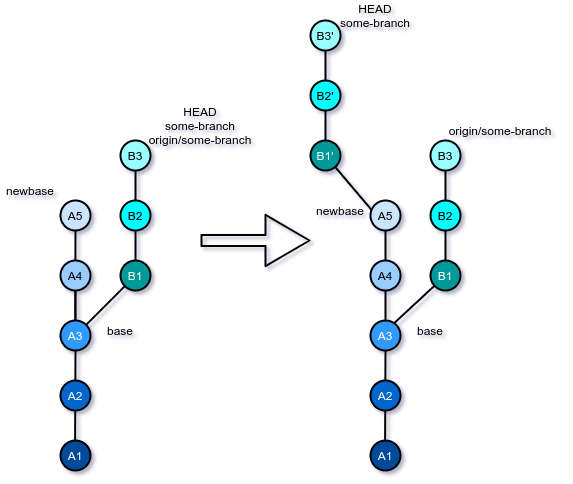
\includegraphics[height=0.65\textheight]{004-rebase}
        \centering
    \end{figure}
\end{frame}

\begin{frame}
    \frametitle{\secname: \small\subsecname\normalsize}

    \begin{itemize}
        \item \textit{Rebase} should be used to move a set of changes from a point to another
        \item Keeps the history clean
        \begin{itemize}
            \item No merge commit except on the main branch
            \item MR only has changes related to that specific MR
            \begin{itemize}
                \item Observed by running \texttt{git diff <base-commit>}
            \end{itemize}
        \end{itemize}
        \item \textbf{Cannot \texttt{git pull} after a rebase!}
        \item Must \texttt{git push --force-with-lease} after rebasing
        \item \texttt{git rebase -i --onto=<newbase> <base>}
        \begin{itemize}
            \item \texttt{-i} stands for "interactive"
        \end{itemize}
    \end{itemize}
\end{frame}
